\subsection{Backend}

Die Dienste wurden mit Eclipse MicroProfile umgesetzt. Neben den standardmäßig enthaltenen Bibliotheken gibt es hierbei aber auch unterstützte optionale Bibliotheken, wie Implementierungen von \texttt{OpenAPI}, \texttt{OpenTracing}, \texttt{Fault Tolerance} und vieler weiterer \cite{EclipseMicroprofile}.

Um Traces von den Microservices zu sammeln, wurde die OpenTracing Implementierung sowie ein Jaeger-Client \cite{JaegerClient} zum Exportieren der Daten hinzugezogen. Mit dieser Anbindung lassen sich per Annotation (vgl. \autoref{lst:implementierung-traced-example}) alle zu tracenden Businessmethoden definieren, die dann automatisch getraced und über den Jaeger-Client an Jaeger gesendet werden. Bei jedem Microservice wurden diese relevanten Methoden annotiert und der Jaeger-Client konfiguriert, was automatisch zu der Übertragung von verteilten Traces in Jaeger führte.

\lstinputlisting[
  language = java,
     style = java-eclipse,
basicstyle = {\footnotesize\fontfamily{pcr}\selectfont},
   caption = Beispielhafter Einsatz der @Traced-Annotation,
captionpos = b,
     label = lst:implementierung-traced-example
]{content/04_erstellung-poc/implementierung-code/TracedExample_OrderService.java}

\begin{wrapfigure}[9]{r}{0.45\textwidth}
\centering
\vspace{-\baselineskip}
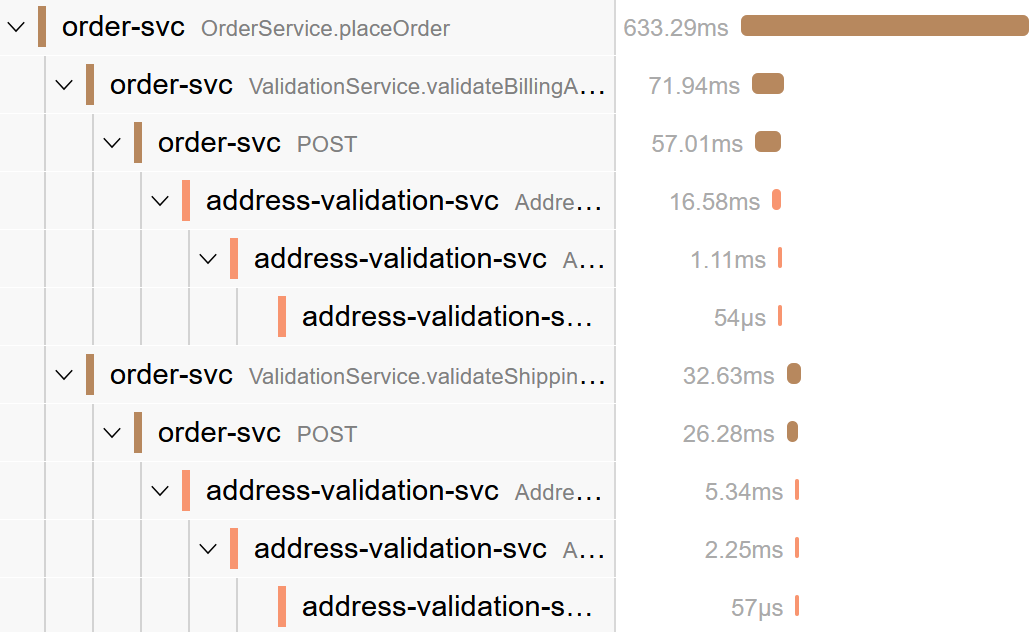
\includegraphics[width=\linewidth]{img/04_erstellung-poc/implementierung_jaeger-trace-example.png}
\caption{Ausschnitt des Traces zu \autoref{lst:implementierung-traced-example}}
\label{fig:implementierung_jaeger-trace-example}
\end{wrapfigure}

In Jaeger erzeugt der o. g. Quellcode die in \autoref{fig:implementierung_jaeger-trace-example} zu sehenden Spans. Bei diesem Ausschnitt ist erkennbar, dass der Dienst \enquote{Bestellungen} für eine ursprüngliche Anfrage zwei Anfragen an den Dienst \enquote{Adressvalidierung} sendet, jeweils für die Rechnungs- und Lieferadresse. Neben den Traces werden keine weiteren Daten von Backend-Komponenten erhoben, da das Hauptaugenmerk der Arbeit auf dem Frontend liegt.

\subsection{Frontend}

\subsubsection{Datenweiterleitung im \enquote{Backend4Frontend}}



Da Logs, Metriken und Fehler mit Splunk gesammelt werden, aber Splunk keine direkt aus dem Browser ansprechbare Schnittstelle bietet, müssen diese über einen Dienst an Splunk weitergeleitet werden (vgl. \autoref{subsec:splunk}). Neben diesen Daten sind zudem Traces auf dem Frontend an Jaeger zu berichten, dies ist aber erneut nicht möglich, da kein browserkompatibler Jaeger-Client identifiziert werden konnte. Eine nähere Betrachtung dessen erfolgt im nächsten Abschnitt.

Da der Dienst \enquote{Backend4Frontend} bereits zum Weiterleiten verwendet wird, wurde dieser erweitert, sodass er Traces, Logs, Metriken sowie Fehler entgegennehmen kann und diese an Jaeger bzw. Splunk sendet. Vor der eigentlichen Weiterleitung werden die Daten mit Kontextinformationen angereichert, wie bspw. der User-IP oder der Browserversion. Die Traces werden dann über eine OpenTelemetry-Anbindung an Jaeger gesendet, die anderen Daten werden an die HEC-Schnittstelle \cite{SplunkHEC} von Splunk übertragen.

\subsubsection{Traces und Metriken}
\label{subsec:traces-und-metriken}

Das Frontend erhebt ebenso wie das Backend Traces, zusätzlich werden aber auch Metriken, Logmeldungen und Fehler erfasst und gemeldet. Traces und Metriken werden auf Basis von OpenTelemetry-JavaScript-Komponenten \cite{OpenTelemetryJS} erhoben. Diese Komponenten werden in einem eigenen Angular-Modul (siehe \autoref{lst:app-observability}) initialisiert und der Anwendung über \enquote{providers} zur Verfügung gestellt. Hierbei wird der SPA ein \texttt{Tracer} bereitgestellt, mit dem Spans aufgezeichnet werden können, ein \texttt{Meter}, welcher es erlaubt Metriken zu erstellen, und eine \texttt{requestCounter}-Metrik, welches die Aufzeichnung der Aufrufanzahl schnittstellenübergreifend erlaubt.

\lstinputlisting[
  language = JavaScript,
     style = ES6,
basicstyle = {\footnotesize\fontfamily{pcr}\selectfont},
   caption = Quellcode des Moduls \enquote{app-observability.module.ts},
captionpos = b,
     label = lst:app-observability
]{content/04_erstellung-poc/implementierung-code/app-observability.module.ts}

Im folgenden \autoref{lst:shopping-cart-datasource} ist die Benutzung des zur Verfügung gestellten \texttt{Tracers} zu sehen, hierbei wird ein Span erstellt und bei Schnittstellenaufrufen an die jeweiligen Services übergeben. Wie der Span weiterverwendet wird, ist im nächsten Absatz beschrieben.

\lstinputlisting[
  language = JavaScript,
     style = ES6,
basicstyle = {\footnotesize\fontfamily{pcr}\selectfont},
   caption = Datenquelle zum Abrufen und Zusammenführen der Artikeldaten,
captionpos = b,
     label = lst:shopping-cart-datasource
]{content/04_erstellung-poc/implementierung-code/tracing_shopping-cart-datasource.ts}

Beispielhaft im Dienst zum Abrufen der Übersetzungsdaten (vgl. \autoref{lst:localization.service}) wird der übergebene Span als Elternspan benutzt. Bei dem eigentlichen HTTP-Aufruf wird zudem ein HTTP-Header \texttt{uber-trace-id} angereichert, den der dort laufende Jaeger-Client interpretiert \cite{JaegerClient} und daraus die Beziehung zu den Frontend-Spans herstellt. Zusätzlich zum Tracing wird hierbei auch die Metrik \texttt{requestCounter} inkrementiert.

\lstinputlisting[
  language = JavaScript,
     style = ES6,
basicstyle = {\footnotesize\fontfamily{pcr}\selectfont},
   caption = Service zum Abrufen der Übersetzungsdaten,
captionpos = b,
     label = lst:localization.service
]{content/04_erstellung-poc/implementierung-code/tracing_localization.service.ts}

Um das Erheben von Traces und Metriken im Frontend zu realisieren, wurden OpenTelemetry-Komponenten herangezogen, da wie in \autoref{subsec:opentelemetry} beschrieben, OpenTelemetry einen vielversprechenden Standard darstellt. Weiterhin konnte keine Bibliothek identifiziert werden, die die Traces erhebt und direkt an Jaeger sendet. Es gibt zwar einen Jaeger-Client für Node.js\footnote{Jaeger-Client für Node.js: \url{https://github.com/jaegertracing/jaeger-client-node}}, jedoch befindet sich das browserkompatible Pendant\footnote{Jaeger-Client für Browser: \url{https://github.com/jaegertracing/jaeger-client-javascript/}} seit 2017 in den Startlöchern \cite{JaegerJSClientUsageInABrowser}. Zudem existiert ein OTel-Exporter für Jaeger\footnote{OTel Jaeger Exporter: \url{https://github.com/open-telemetry/opentelemetry-js/tree/main/packages/opentelemetry-exporter-jaeger}}, welcher jedoch auch nur mit Node.js funktioniert. Grund hierfür ist, dass das zugrundeliegende Protokoll gRPC \cite{grpc} nicht komplett aus einer Browserumgebung aus unterstützt wird \cite{grpcWebLimitations}.

\nomenclature[Fachbegriff]{gRPC}{gRPC Remote-Procedure-Call}

Die gesammelten OTel-Tracingdaten werden über einen Standard-Exporter an das \enquote{Backend4Frontend} gesendet, welcher diese dann in ein Jaeger-konformes Format umwandelt und sie dann subsequent an Jaeger übertragt. Die Metrikdaten werden bereits im Frontend in ein Splunk-kompatibles Logformat konvertiert. Nach der Konvertierung werden die Daten an den \texttt{SplunkForwardingService} übergeben, welcher in \autoref{subsec:weiterleitung-an-splunk} näher beschrieben wird.

\subsubsection{Logging}

Das Logging im Frontend wurde über das npm \cite{NPM} Paket \texttt{ngx-logger}\footnote{ngx-logger auf GitHub: \url{https://github.com/dbfannin/ngx-logger}} realisiert, welches eine speziell an Angular angepasste Logging-Lösung darstellt. Da dieses Paket extra an Angular angepasst ist, lässt es sich ohne großen Aufwand als Modul einbinden und einsetzen (vgl. \autoref{lst:logging_app.module}).

\lstinputlisting[
  language = JavaScript,
     style = ES6,
basicstyle = {\footnotesize\fontfamily{pcr}\selectfont},
   caption = Ausschnitt des Hauptmoduls \texttt{app.module.ts},
captionpos = b,
     label = lst:logging_app.module
]{content/04_erstellung-poc/implementierung-code/logging_app.module.ts}

Wie in den vorherigen Codebeispielen zum Tracing zu sehen war, kann ein \texttt{NGXLogger} im Konstruktor von Komponenten und Diensten injected werden. Logmeldungen, die hiermit erfasst werden, werden je nach Konfiguration und Loglevel der jeweiligen Meldung in die Browserkonsole geschrieben. Über einen \texttt{NGXLoggerMonitor} lassen sich die Logmeldungen anzapfen, wie in \autoref{lst:splunk-logging-monitor} zu sehen ist. Hierbei werden die Logmeldungen in ein Splunkformat übertragen und dann über den \texttt{SplunkForwardingService} an das \enquote{Backend4Frontend} übertragen. Die Funktionsweise der Weiterleitung wird an späterer Stelle genauer beschrieben.

\lstinputlisting[
  language = JavaScript,
     style = ES6,
basicstyle = {\footnotesize\fontfamily{pcr}\selectfont},
   caption = Implementierung des \texttt{NGXLoggerMonitor}-Interfaces,
captionpos = b,
     label = lst:splunk-logging-monitor
]{content/04_erstellung-poc/implementierung-code/splunk-logging-monitor.ts}

\subsubsection{Fehler}

Die ErrorHandler-Hook von Angular übermittelt aufgetretene und unbehandelte Fehler an den \texttt{SplunkForwardingErrorHandler}. Weiterhin ist der ErrorHandler ein \texttt{Injectable}, wodurch er in andere Angular-Klassen \enquote{injected} werden kann. Der ErrorHandler wird bspw. bei den Schnittstellen dazu verwendet, um dort bereits behandelte Fehler auch an Splunk zu übermitteln.

Wird ein Fehler gemeldet, werden zunächst die Fehlerinformationen in einen Splunk\-da\-ten\-satz konvertiert und dann über den \texttt{SplunkForwardingService} weitergeleitet. Neben diesem Verhalten wird zusätzlich auch der Fehler an LogRocket übermittelt, damit dieser im Video des Session-Replays gesondert angezeigt wird.

\lstinputlisting[
  language = JavaScript,
     style = ES6,
basicstyle = {\footnotesize\fontfamily{pcr}\selectfont},
   caption = ErrorHandler zum Abfangen und Weiterleiten von aufgetretenen Fehlern,
captionpos = b,
     label = lst:splunk-forwarding-error-handler
]{content/04_erstellung-poc/implementierung-code/splunk-forwarding-error-handler.ts}

\subsubsection{Weiterleitung an Splunk}
\label{subsec:weiterleitung-an-splunk}

Logs, Metriken und Fehler über den  \texttt{SplunkForwardingService} an das \enquote{Backend\-4\-Frontend} gesendet und letztendlich an Splunk übermittelt. Damit nicht jedes Datenobjekt einen Aufruf auslöst, gruppiert dieser \texttt{Service} die eintreffenden Daten.

Im \autoref{lst:splunk-forwarding.service} ist erkennbar, dass alle 5s geprüft wird, ob Daten zur Weiterleitung zur Verfügung stehen. Ebenso ist zu sehen, dass beim Fehlschlag des Sendens eines Batches, fünf Wiederholversuche gestartet werden, mit einer Wartezeit von 15s. Die grundlegende Funktionalität dessen wurde mit RxJS \cite{RxJS} umgesetzt, einer Kernbibliothek von Angular, die Reactive Programming \cite{ReactiveProgramming} in JavaScript erlaubt. Weiterhin werden die Daten an Splunk nicht im Textformat übertragen, sondern direkt in JSON. Die JSON-Objekte werden automatisch von Splunk interpretiert und die enthaltenen Felder zugreifbar gemacht. Durch das gewählte Format \cite{StructuredAndInteroperableLogging} ist auch die \autoref{anf:3200} zum Structured-Loggings erfüllt. Ausgesuchte Logmeldungen und Fehler sind in \autoref{lst:log-batch_example} zu betrachten.

\lstinputlisting[
  language = JavaScript,
     style = ES6,
basicstyle = {\footnotesize\fontfamily{pcr}\selectfont},
   caption = Implementierung des \texttt{SplunkForwardingService},
captionpos = b,
     label = lst:splunk-forwarding.service
]{content/04_erstellung-poc/implementierung-code/splunk-forwarding.service.ts}

\pagebreak

\lstinputlisting[
  language = JSON,
basicstyle = {\footnotesize\fontfamily{pcr}\selectfont},
   caption = Beispiel eines Batches,
captionpos = b,
     label = lst:log-batch_example
]{content/04_erstellung-poc/implementierung-data/log-batch_example.json}

\subsubsection{Session-Replay}

\begin{wrapfigure}[9]{r}{0.35\textwidth}
\centering
\vspace{-0.5\baselineskip}
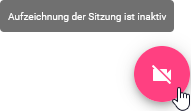
\includegraphics[width=\linewidth]{img/04_erstellung-poc/implementierung_frontend_recording-consent_button-inactive.png}
\caption{Button zum Öffnen des Dialogs}
\label{fig:recording-consent_button-inactive}
\end{wrapfigure}

Die Übermittlung der Daten an LogRocket wird erst aktiviert, wenn der Nutzer explizit der Aufzeichnung zustimmt. Dies bedeutet jedoch auch, dass bis zur Zustimmung keine Sitzungsdaten aufgenommen wurden. Klickt der Nutzer jedoch auf den, unten rechts in der Anwendung schwebenden, Button (vgl. \autoref{fig:recording-consent_button-inactive}), wird ein Einverständnis-Dialog geöffnet. Hierbei (vgl. \autoref{fig:recording-consent_dialog-inactive}) erhält der Nutzer eine Übersicht welche Daten aufgenommen werden und an wen diese dann weitergesendet werden. Stimmt der Nutzer zu, wird LogRocket initialisiert, wie im \autoref{lst:record-consent-dialog.component.html} sowie \autoref{lst:record-consent-dialog.component.ts} zu sehen ist. Nach dem Warenkorbdialog und nach der Eingabe der Rechnungsadresse werden zudem weitere identifizierende Daten an LogRocket übermittelt. Die Aufnahme der Sitzung läuft größtenteils autonom, lediglich behandelte Fehler müssen LogRocket manuell übermittelt werden.
	
\begin{figure}[H]
	\centering
	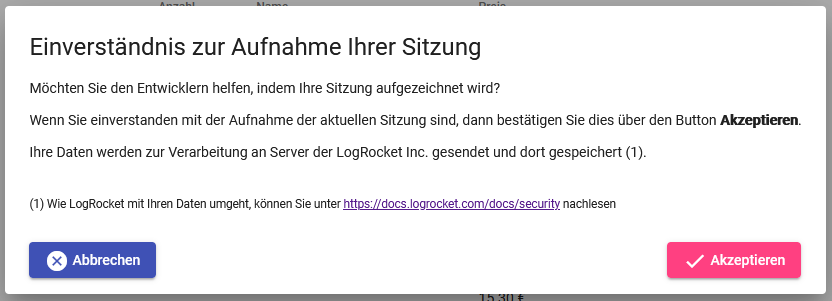
\includegraphics[width=1.00\linewidth]{img/04_erstellung-poc/implementierung_frontend_recording-consent_dialog-inactive.png}
	\caption{Einverständnis-Dialog}
	\label{fig:recording-consent_dialog-inactive}
\end{figure}

\vspace{-0.5\baselineskip}

\lstinputlisting[
  language = AngularTemplateHTML,
basicstyle = {\footnotesize\fontfamily{pcr}\selectfont},
   caption = Angular HTML-Template der Einverständnis-Komponente,
captionpos = b,
     label = lst:record-consent-dialog.component.html
]{content/04_erstellung-poc/implementierung-code/record-consent-dialog.component.html}

\lstinputlisting[
  language = JavaScript,
     style = ES6,
basicstyle = {\footnotesize\fontfamily{pcr}\selectfont},
   caption = Initialisierung von LogRocket in der Einverständnis-Komponente,
captionpos = b,
     label = lst:record-consent-dialog.component.ts
]{content/04_erstellung-poc/implementierung-code/record-consent-dialog.component.ts}

\subsection{Architektur}

Abschließend lässt sich somit folgende, in \autoref{fig:implementierung_architektur} zu betrachtende, Architektur visualisieren. Bei \circled{1} lässt sich die Übertragung von Spans an Jaeger betrachten, bei dem die Backend-Dienste aufgrund der verwendeten Java-Anbindung (\texttt{io\allowbreak{}.\allowbreak{}jaegertracing\allowbreak{}:\allowbreak{}jaeger-client}) die Spans über das Protokoll \enquote{Apache Thrift} \cite{Thrift} berichten und das \enquote{Backend4Frontend} verwendet zur Weiterleitung eine OTel-Anbindung an Jaeger, die wiederum gRPC verwendet. Die Übertragung von Log-, Metrik sowie Fehlerdaten lässt sich bei \circled{2} betrachten. Dabei handelt es sich um Daten, die zuvor vom Frontend gesendet wurden (vgl. \circled{3}). Die Kommunikation mit LogRocket (vgl. \circled{4}) verläuft ohne Weiterleitung und mit einem proprietärer Protokoll auf Basis von gRPC \cite{LogRocketPerformance}.

\pagebreak

\begin{figure}[H]
	\begin{adjustbox}{addcode={
		\begin{minipage}{\width}}{
			\caption{Architektur des Proof-of-Concepts. Eigene Darstellung}
			\label{fig:implementierung_architektur}
		\end{minipage}},rotate=90,center}
		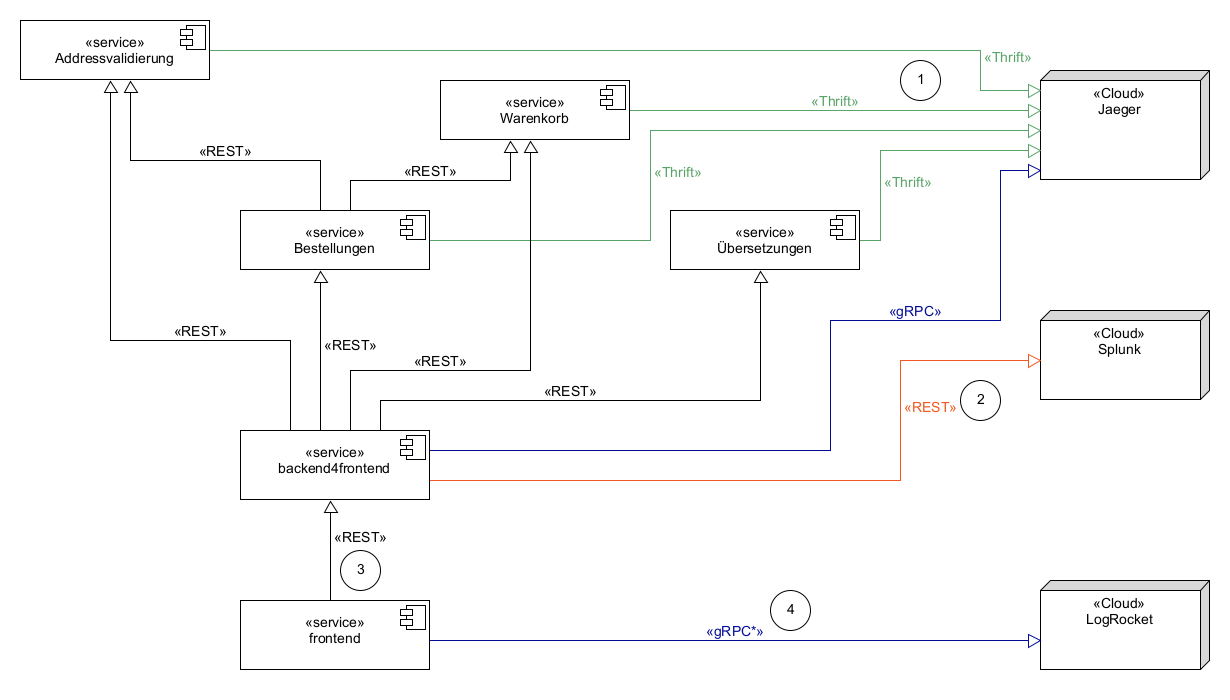
\includegraphics[height=0.80\textwidth]{img/04_erstellung-poc/implementierung.png}
	\end{adjustbox}
\end{figure}

\pagebreak